\chapter{Transport Layer}

\section{Introduzione al Transport Layer}
Il transport layer è situato tra l'application e il network layer. I protocolli di questo livello, permettono all'application layer di usufruire di una \textbf{connessione logica tra processi}, e quindi di una comunicazione \textbf{end-to-end}. 

\subsection{Connessione logico, connessione reale}
Introducendo il concetto di \textbf{protocollo}, abbiamo capito che questi forniscono delle specifiche di "incapsulamento" e delle specifiche di "interpretazione" dei dati. Inoltre, abbiamo capito che in termini esclusivamente \textbf{logici}.,  l'$i$-esimo layer di un host $A$, comunica direttamente con l'$i$-esimo layer dell'host $B$. $A$ incapsula i dati con header opportuni, $B$ interpreta in maniera opportuna seguendo le indicazioni del protocollo e degli header.\\
Ogni layer ha un ruolo specifico, in particolare:
\begin{itemize}
	\item Il \textbf{livello di trasporto} crea una \textbf{connessione logica tra processi}.
	\item Il \textbf{livello di rete}, crea una \textbf{connessione logica tra host}.
	\item Il \textbf{livello di collegamento} (Data Link) si occupa della \textbf{comunicazione fisica} tra due host (fisicamente) collegati.
\end{itemize}

\begin{figure}[htp]
	\centering
	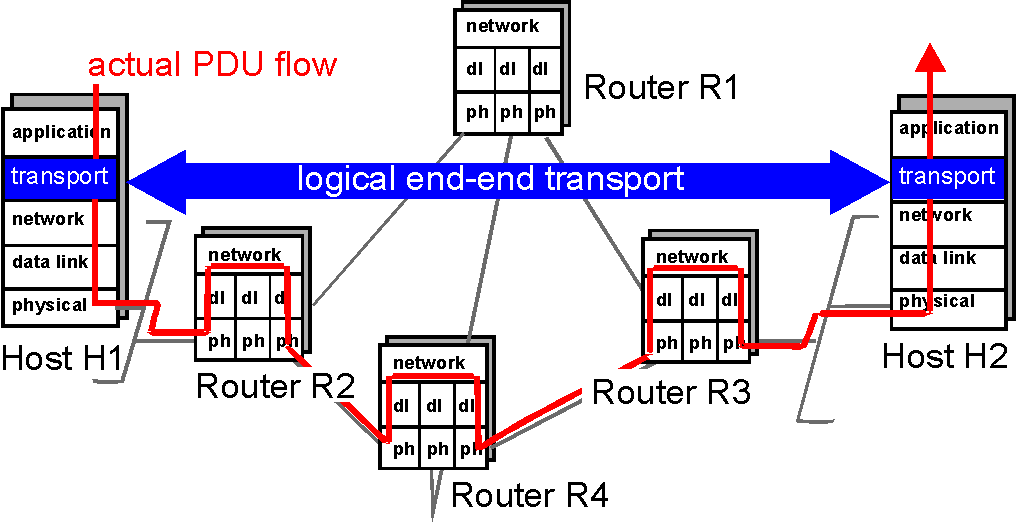
\includegraphics[width=0.75\linewidth]{./images/connessione.png}
	\caption{Trasferimento logico vs effettivo}
\end{figure}

\newpage

Nonostante la comunicazione \textbf{end-to-end logica} tra il transport layer degli host coinvolti esista, nella pratica la questione è ben più complessa: ogni protocollo di un dato livello, sfrutta infatti i protocolli dei livelli inferiori (come da disegno) per trasmettere con successo. Segue un esempio:

\begin{enumerate}
	\item Un host desidera mandare una richiesta HTTP. Crea il messaggio HTTP secondo il protocollo dell'application layer.
	\item Passa il messaggio HTTP al livello di trasporto, che lo incapsula in un segmento TCP.
	\item Il livello di trasporto, passa il segmento al livello di rete, che lo incapsula in un pacchetto (o datagramma) IP.
	\item Infine, il livello Data Link, si occupa di incapsulare in un frame il pacchetto fornito dal livello di rete.
	\item Avviene la trasmissione.
\end{enumerate}

Al sender, corrisponderà una sequenza di passaggi simili, ma dal basso verso l'alto, con un decapsulamento guidato dalle informazioni degli header, che permetteranno ad ogni layer di interpretare correttamente i dati ricevuti. Per ora, non approfondiamo nemmeno quanto l'inoltro da un router all'altro complichi la sitauzione! 


\section{Multiplexing e Demultiplexing}
Sono le tecniche utilizzate dal livello di trasporto, per garantire che \textbf{il trasporto da host a host}, fornito dal livello di rete, diventi una comunicazione \textbf{da processo a processo}.

\subsection{Multiplexing}
Il \textbf{multiplexing avviene al mittente}, è il processo con cui un host incapsula i frammenti di dati provenienti da uno o più sockets in \textbf{segmenti del transport layer} con opportuni header, che verranno poi usati in fase di demultiplexing dal receiver.

\subsection{Demultiplexing}
\textbf{Il demultiplexing vviene al destinatario}. Consiste nella \textbf{consegna dei segmenti al socket corretto}, e quindi al processo corretto, sfruttando le specifiche degli header, tra cui, chiaramente, la porta.

\begin{figure}[htp]
	\centering
	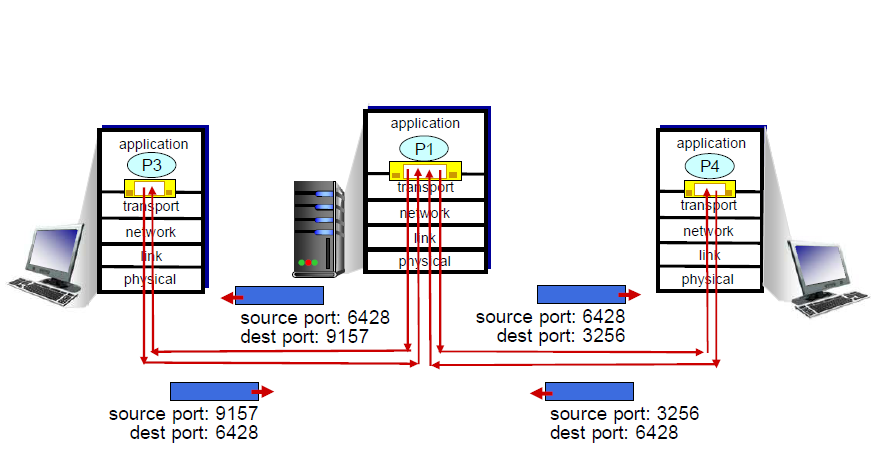
\includegraphics[width=0.75\linewidth]{./images/demultiplexing.png}
	\caption{Esempio di demultiplexing connectionless}
\end{figure}
\begin{figure}[htp]
	\centering
	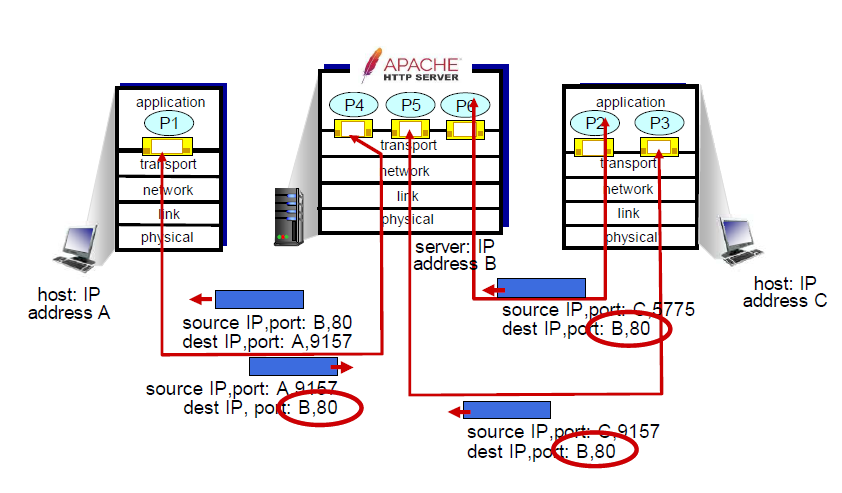
\includegraphics[width=0.75\linewidth]{./images/demultiplexingconnection.png}
	\caption{Esempio di demultiplexing connection-oriented}
\end{figure}

\newpage

\section{UDP - User Datagram Protocol}
TCP e UDP sono indubbiamente i \textbf{protocolli di trasporto dati} più popolari. Se il TCP è noto per la sua affidabilità (tramite i meccanismi di ACK da esso implementati), lo stesso non si può dire di UDP. Nonostante ciò, le funzionalità ridotte di UDP garantiscono un protocollo \textit{bare bones}, ridotto all'osso, \textbf{molto più veloce} e con meno \textit{overhead}.

\subsection{Caratteristiche di UDP}

\begin{itemize}
	\item È un protocollo di trasporto \textbf{bare-bones}, leggero, ma unreliable.\\ 
	Nessun handshake avviene tra il mittente e il destinatario. Ogni segmento UDP è gestito in maniera indipendente dagli altri, e non esistono vere e proprie "sessioni UDP". Per questo, è definito come un protocollo \textbf{connectionless}.
	
	\item L'header del protocollo UDP occupa 8 byte. 2 byte per la porta del mittente, 2 per la porta del destinatario, 2 per la lunghezza del messaggio (header UDP + dati) e 2 per il checksum. L'header  del protocollo TCP occupa dai 20 ai 60 byte: ben di più rispetto a UDP!
	
	\item È usato da applicazioni di streaming multimediale, comunicazione VoiP e DNS.  Si presta ad applicazioni che riescono a lavorare anche con \textbf{perdite di pacchetti}.
\end{itemize}

\subsection{Checksum (per UDP, ma anche TCP)}
È un meccanismo che consente di \textbf{rilevare errori di trasmissione}. Questi errori spesso consistono in \textbf{bit-flip}, che possono stravolgere del tutto i l significato dei dati trasmessi. Detto ciò, la verifica consiste nel calcolo di un \textbf{checksum}, in italiano \textbf{somma di controllo}, sia al mittente (che la inserirà nel frame) che al destinatario. La somma è calcolata in virtù dei dati contenuti nel frame. Se le due somme non dovessero coincidere, il pacchetto sarà da considerarsi fallato, e verrà scartato. 

\newpage

\section{Reliable Data Transfer - Trasferimento affidabile}
Data una rete di dispositivi comunicanti, quello che spesso si potrebbe pensare, è che la comunicazione sia sempre, a priori, affidabile. - \textit{Ogni pacchetto inviato arriva al mittente!} - E invece no. \textbf{Il canale di comunicazione è da considerarsi inaffidabile}, per una serie di motivi legati alla natura fisica del canale, ma anche a causa della "consapevolezza" limitata degli host: due host non conoscono reciprocamente i loro stati, se non comunicando. E se dei pacchetti si perdono? Nonostante ciò, tramite software, è possibile garantire un \textbf{trasporto affidabile} che rende più \textbf{robusta} la comunicazione. \textit{Creare un canale di comunicazione affidabile partendo da un canale fisico inaffidabile} è l'obiettivo posto dal topic \textbf{Reliable Data Transfer}.


\subsection{RDT - Introduzione}
Reliable Data Transfer è un meccanismo, descritto tramite \textbf{macchine a stati finiti}, che offre, nelle sue versioni, delle soluzioni software (per sender e receiver) per creare da canali fisici inaffidabili, connessioni affidabili. I meccanismi descritti da RDT, sono gli stessi seguiti da alcuni dei protocolli del livello di trasporto (banalmente, TCP).
\begin{figure}[htp]
	\centering
	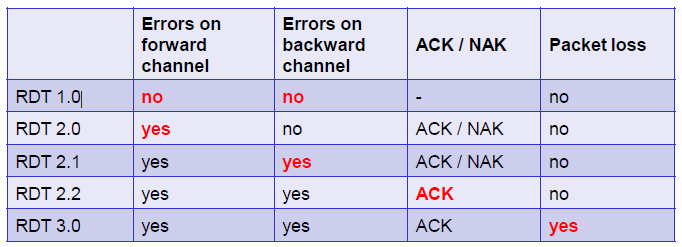
\includegraphics[width=0.5\linewidth]{./images/rdtversions.png}
	\caption{Versioni di RDT}
\end{figure}

Osserviamo in breve le caratteristiche dei vari RDT prima di studiarne le FSM al dettaglio:
\begin{itemize}
	\item 1.0. Non include nessun meccanismo effettivo, ma fa da base per le versioni successive.
	\item 2.0. Gestisce i pacchetti corrotti tramite segnali di ACK/NAK, ma non gestisce ACK e NAK corrotti.
	\item 2.1. Gestisce gli errori sul backward channel\footnote{Il backward channel è canale per l'invio dei segnali di ACK/NAK durante una connessione.}.
	\item 2.2. Si elimina il simbolo dedicato NAK, utilizzando in maniera differente gli ACK.
	\item 3.0. Tutte le precedenti versioni gestiscono solo pacchetti corrotti. Con questa versione, si verifica anche la perdita dei pacchetti, introducendo il meccanismo di time-out.
\end{itemize}


\subsection{RDT 1.0 - Canale perfetto, zero errori, zero perdite}
Presuppone un \textbf{canale perfetto} senza errori di bit e perdita di pacchetti. Sarà la base per le successive versioni di RDT.
Gli automi rimangono in attesa di un certo evento. La verifica dell'evento avviene tramite il cosiddetto "polling" o interrogazione.\\
Il \textbf{polling rate} stabilisce ogni quanto interrogare la condizione. Il polling rate DEVE essere stabilito, in quanto, altrimenti la verifica avverrebbe un numero di volte pari alla frequenza della CPU,  e si avrebbero comportamenti anomali.
\begin{figure}[htp]
	\centering
	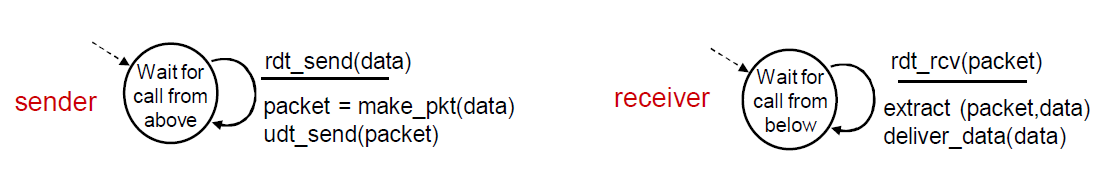
\includegraphics[width=1\linewidth]{./images/fsmrdt1.png}
\end{figure}
La FSM del sender si attiva quando riceve una richiesta per mandare dei dati. Quella del receiver, quando riceve dei pacchetti. \verb|deliver_data(data)| si riferisce a socket. 

\newpage

\subsection{RDT 2.0 - Canale imperfetto, errori sul forward}
Introduce \textbf{un checksum} e un \textbf{meccanismo di ACK} (senza checksum). Il sender manda un pacchetto e aspetta un feedback. \\ Si ipotizza che non si perdano pacchetti e che il backward sia perfetto. 

\begin{figure}[htp]
	\centering
	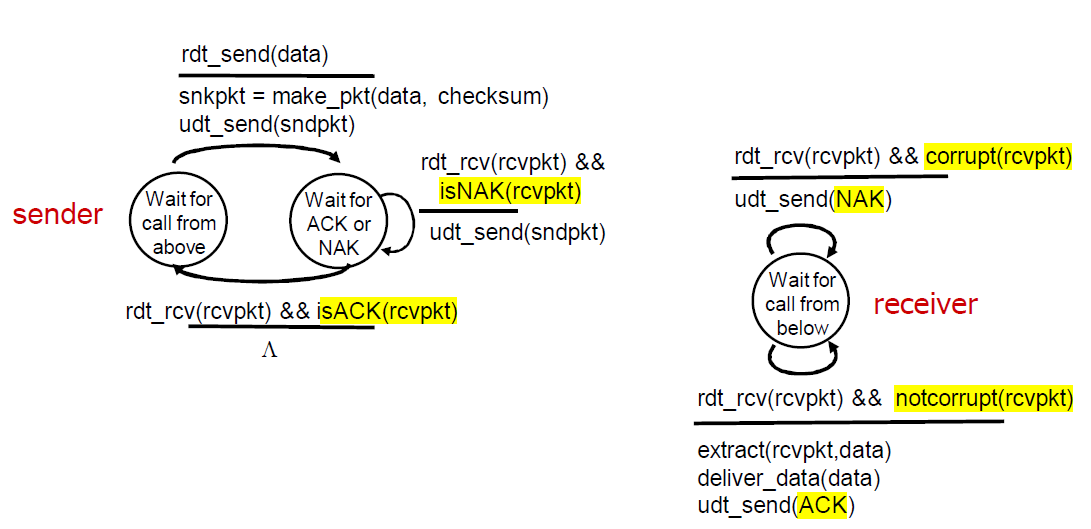
\includegraphics[width=1\linewidth]{./images/fsmrdt2.png}
\end{figure}


\begin{itemize}
	\item Il sender che ha appena mandato il pacchetto attende un ACK o un NAK.
	\item Il receiver verifica se il pacchetto è corrotto o meno, e in caso, manda un NAK o un ACK.
	\item Se il sender riceve ACK, ritorna allo stato iniziale ($\Lambda$), altrimenti rimanda il pacchetto arrivato corrotto.
\end{itemize}

Ipotizzare che il backward sia perfetto, è che ACK e NAK arrivino sempre integri, è azzardato: un ACK potrebbe corrompersi, diventare un NAK o non arrivare mai. Un hacker potrebbe sfruttare questa debolezza sostituendo tutti i pacchetti ACK con un NAK o un pacchetto differente, secondo l'approccio \textbf{Man-In-The-Middle}.

\newpage
\subsection{RDT 2.1 - Errori sul forward e sul backward}
L'RDT 2.1 nasce dall'esigenza di gestire un backward channel imperfetto, integrando un \textbf{checksum sugli ACK/NAK}. A ogni pacchetto viene annesso un \textbf{bit sequenza}, per disambiguare i pacchetti e gli ACK. A ogni pacchetto mandato, il sender integra un bit che si alterna tra 0 e 1. Quando il sender riceve un ACK/NAK corrotto, rimanda il pacchetto. Se il receiver riceve due volte lo stesso pacchetto con lo stesso bit sequenza, sa di dover \textbf{rimandare l'ACK}.

\subsubsection{Sender}
\begin{figure}[htp]
	\centering
	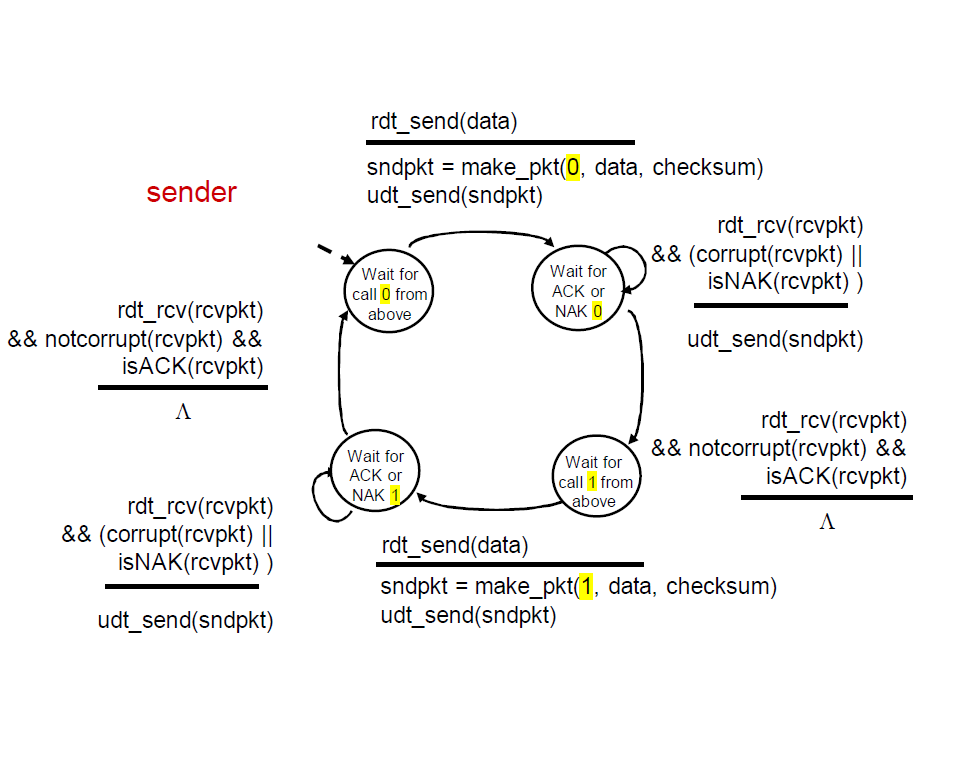
\includegraphics[width=0.8\linewidth]{./images/fsmrdt2.2sender.png}
\end{figure}

\subsubsection{Receiver}
\begin{figure}[htp]
	\centering
	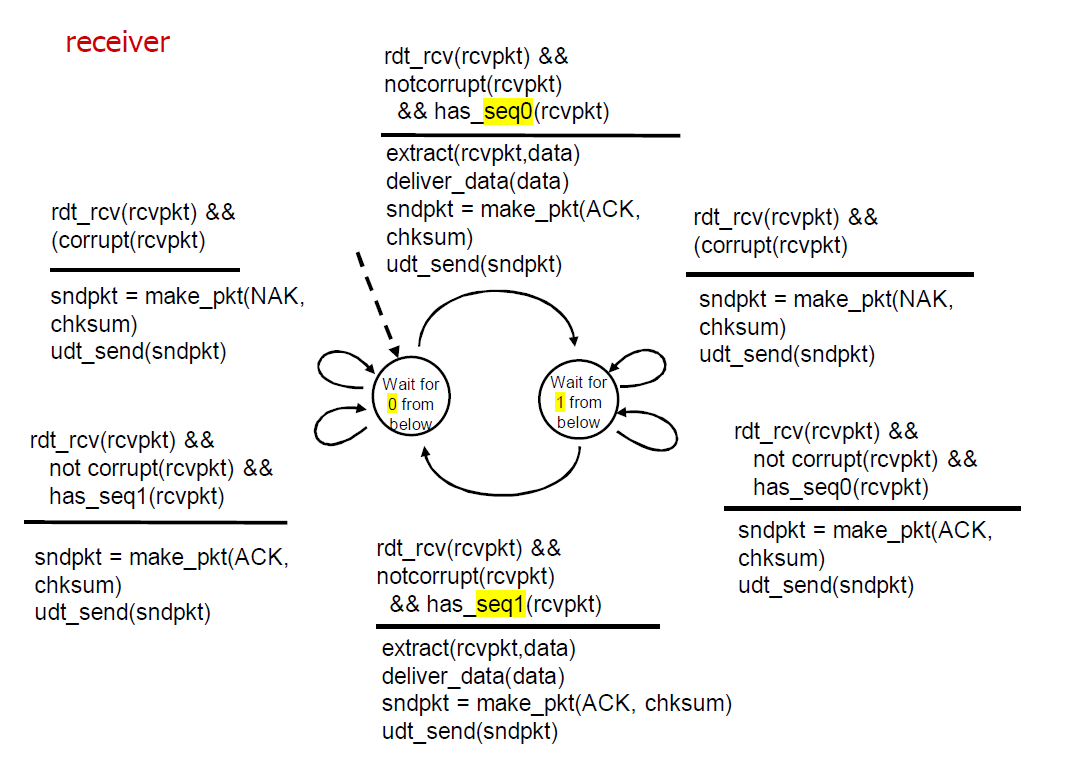
\includegraphics[width=0.8\linewidth]{./images/fsmdrt2.2receiver.png}
\end{figure}

\newpage

\subsection{RDT 2.2 - Eliminiamo il NAK!}
Rimuove il segnale NAK, cambiando leggermente il funzionamento dell'ACK:
\begin{itemize}
	\item Se il \textbf{pacchetto è stato consegnato correttamente}, viene mandato il segnale di \\ACK \underline{relativo al pacchetto}.
	\item Se il pacchetto \textbf{non è stato consegnato correttamente}, viene mandato il segnale di ACK \underline{dell'ultimo pacchetto ricevuto correttamente}.
\end{itemize}

\begin{figure}[htp]
	\centering
	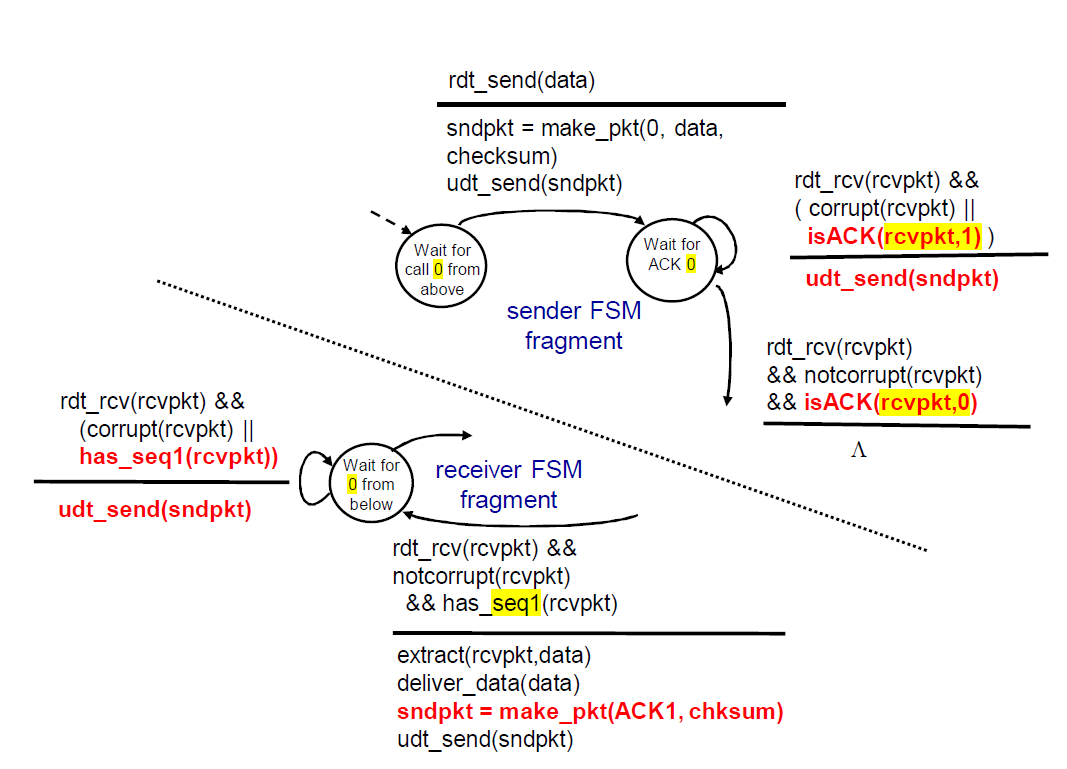
\includegraphics[width=1\linewidth]{./images/fsmdrt2.2.png}
\end{figure}
Nelle versioni precedenti, il NAK e l'ACK sono due segnali differenti. Un segnale che non è né ACK né NAK, a causa di una distorsione del segnale o un bit-flip, porta a dei segnali che il sistema non sa come gestire. \textbf{Rimuovere la classe dei segnali NAK ci permette di non cadere in} queste \textbf{ambiguità}.\\
Tuttavia, non contempliamo ancora la perdita di pacchetti.
\newpage

\subsection{RDT 3.0 - Errori e perdite}
Assumiamo (finalmente) che il canale possa perdere pacchetti (sia dati, che ACKs).\\ Gestiamo il tutto con la \textbf{temporizzazione}.

\subsubsection{Sender}
\begin{figure}[htp]
	\centering
	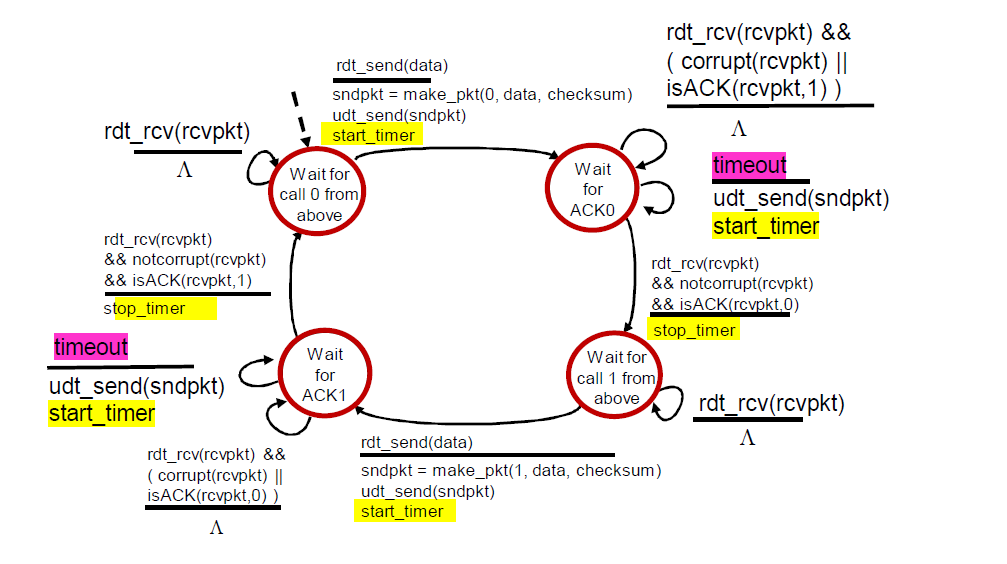
\includegraphics[width=1\linewidth]{./images/fsmrdtsender.png}
\end{figure}

\subsubsection{Receiver}
Macchina a stati finiti analoga a quella di RDT 2.2. La temporizzazione è gestita esclusivamente al sender.

\newpage

\section{Calcolo del Throughput}
Il \textbf{throughput} è un'indice della capacità di trasmissione di un canale di comunicazione. 

$$
\text{Throughput} = \frac{\text{Numero di bit (o byte) trasmessi con successo}}{\text{Tempo impiegato}}
$$

\subsection{Throughput teorico}
Consideriamo un canale con \textbf{Bandwidth} $BW = 10 \text{ Mbps}$ (Megabit per secondo).
Questo vuol dire in un secondo possono essere trasmessi $10^7$ bit. Un bit viene 
trasmesso in $\frac{1}{10^7} = 0.1 \mu s$ (microsecondo).

\subsubsection{Tempo di trasmissione di un frame}
Consideriamo ora di voler trasmettere un frame di 1500 byte, ovvero $1500 \cdot 8 = 12000$ bit.\\
Per trasmettere un frame, impieghiamo il seguente tempo:
$$
T_\text{frame} = \frac{\text{Dimensione del frame (in bit)}}{\text{Bandwidth (in bit/s)}} = \frac{12000 \ bit}{10^7 \ bit/s} = 0.0012s  = 1200 \mu s  
$$

\subsubsection{Tempo di propagazione}
Nella trasmissione dobbiamo anche considerare il tempo di propagazione, che è il tempo richiesto al segnale per arrivare fisicamente da host $A$ a $B$: supponiamo che lo spazio di trasmissione sia pari ad $1km$. 
Supponiamo che la velocità di trasmissione, che dipende dal mezzo che usiamo e dalle sue condizioni, sia  $v \approx 200.000km/s$, e che sia un valore costante.
Il tempo di propagazione è dato dal rapporto spazio/velocità.

$$
T_\text{propagazione} = \frac{\text{Spazio di trasmissione}}{\text{Velocità di trasmissione}} = \frac{1km}{200000 km/s} = \frac{1}{200000} s = 5\cdot 10^{-6} s =  5 \mu s
$$

Con questa informazione possiamo anche andare a calcolare il numero di bit che possono occupare il canale contemporaneamente, ovvero
$$
\text{Bandwidth (in bit/s)}\cdot T_\text{propagazione}\text{(in s)} = 10^7\text{ bit/s} \cdot 5 \cdot 10^{-6}\text{ s} = 50 \text{ bit}
$$

\subsubsection{Tempo di trasferimento}
Ora abbiamo tutte le informazioni necessarie per calcolare il tempo di trasferimento complessivo.\\
Esso indica il tempo che il frame necessita per essere trasferito (ipotizzando che non ci siano da considerare variabili relative ai tempi di connessione, ACK, etc.).

$$
T_\text{trasferimento} = T_\text{frame} + T_\text{propagazione} = 1200 \mu s + 5 \mu s = 1205 \mu s
$$

\begin{figure}[htp]
	\centering
	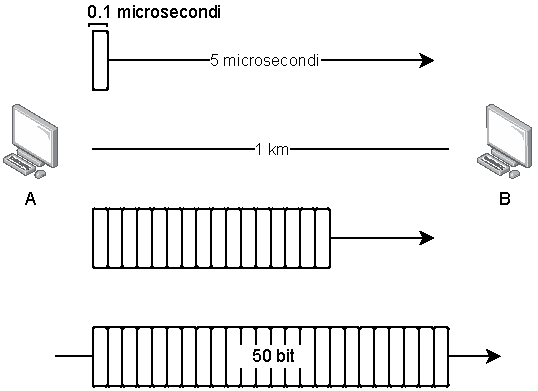
\includegraphics[width=0.65\linewidth]{./images/throughput.pdf}
\end{figure}

\newpage

\subsection{Throughput effettivo}
Quello appena calcolato, è da definirsi un \textbf{througput teorico}. Il \textbf{throughput effettivo} è influenzato anche da altri elementi di attesa, quali \textit{Round Trip Time}, tempi di elaborazione e di trasferimento relativi agli \textbf{ACK}.

\subsubsection{RTT - Round Trip Time}
Il Round Trip Time può essere stimato, e dedicheremo una sezione proprio alle metodologie di stima. È definito come il tempo che intercorre tra l'inizio dell'invio di un messaggio, e la ricezione della sua conferma.

\subsubsection{Tempo di trasmissione ACK}
Il segnale di ACK ha solitamente dimensione pari a $64 \ byte = 64 \cdot 8 \ bit = 512 \ bit$. Ne consegue che:
$$
T_{ACK} = \frac{\text{Dimensione dell'ACK (in bit)}}{\text{Bandwidth (in bit/s)}} = \frac{512}{10^7} = 0.0000512 s = 51.2  \mu s 
$$

\subsubsection{Tempo di trasferimento effettivo}

Stimiamo un tempo di elaborazione dell'ACK di $3 \mu s$ e un RTT di $10 \mu s$ ($5\mu s \cdot 2$, ovvero il $T_{propagazione}$, ma in andata e ritorno).
Otteniamo quindi un tempo complessivo pari a:

$$
T_\text{effettivo} = T_{frame} + T_{ACK} + RTT + \text{Elaborazione ACK} = 1200 + 51.2 + 10  + 3 =  1264.2 \mu s
$$

\subsubsection{Calcolo del Throughput effettivo}
Calcoliamo ora il throughput effettivo, mettendo a rapporto il numero di bit per frame da trasmettere con il tempo di trasferimento totale

$$
\frac{\text{Dimensione del frame (in bit)}}{\text{Tempo totale di trasmissione (in s)}} = \frac{12000}{1264.2 \cdot 10^{-6}} = 9.492 \text{ Mbps}
$$

Osserviamo con piacere che otteniamo un valore molto simile alla larghezza di banda. I fattori esterni non hanno creato particolari \textbf{colli di bottiglia} alla nostra capacità di trasmissione! Il mezzo è ben sfruttato.

\subsubsection{Conclusioni sul throughput reale}
Il throughput reale è fortemente influenzato dal tempo di elaborazione dei segnali di ACK e dall'RTT. Nel caso appena studiato, la \textbf{bandwidth è ben sfruttata}, ma quando l'RTT sarà dell'ordine dei millisecondi\footnote{Recap sui prefissi: milli- = $10^{-3}$, micro- = $10^{-6}$, nano- = $10^{-9}$, kilo- = $10^{3}$, mega- = $10^{6}$, giga- = $10^{9}$;}, e non dei microsecondi, otterremo dei cali di performance non da poco. 




\subsection{Considerazioni}
Il \textbf{tempo di propagazione} è il tempo richiesto ad un segnale per trasmettersi da un punto all'altro. Precedentemente, abbiamo stimato l'$RTT$ come due volte il $T_{propagazione}$. Nel protocollo TCP è presente il meccanismo di Three Way Handshake: questo implica ulteriore ritardo per l'RTT, che può di gran lunga superare la stima calcolata. Se i valori sono diversi, nel calcolo, andremo a considerare il maggiore tra i due.\\
Inoltre, se la bandwidth effettiva calcolata è superiore a quella teorica, allora la bandwidth teorica funge da collo di bottiglia: la bandwidth effettiva sarà uguale a quella teorica, in quanto limite massimo.

\subsection{Ping}
Il comando \verb|ping| è un utility che permette di calcolare l'RTT necessario per la connessione ad un server, e fornisce anche la percentuale di pacchetti persi. Usa il protocollo ICMP.

\newpage


\section{Modalità Pipeline}
È una modalità che consente di aumentare il throughput di una rete. Invece di inviare un singolo frame e aspettare il rispettivo ACK (modalità esposta in precedenza, nota come modalità \textbf{stop-and-wait}), si stabilisce una window di $n$ frame di cui si \textbf{potranno aspettare gli ACK contemporaneamente}. Questo\textbf{ riduce di molto l'influenza del $RTT$ sul throghput}, riducendo di molto l'\textit{overhead} delle singole trasmissioni. L'utilizzo della modalità pipeline è chiaramente più \textbf{vantaggiosa della stop-n-wait}, soprattutto nel contesto di \textbf{reti ad alta latenza}. La finestra d'invio verrà succesivamente indicata con il nome \verb|cwnd|, nel contesto del controllo della congestione.

\subsubsection{Esempio}
Vogliamo mandare pacchetti di 1000 byte.\\
$BW = 1 Gbps = 1000 \ Mbps = 1\cdot10^{9} \ bps$.\\
$RTT=30 \ ms$.\\
Il tempo teoricamente richiesto sarebbe

$$
T_{frame} = \frac{\text{Dimensione dati (in bit)}}{\text{Bandwidth (in bit/s)}} = \frac{8\cdot 10^3 \text{ bit}}{1\cdot10^9 \text{ bit/s}}= 8\cdot 10^{-6} \ s = 8 \mu s
$$
a cui aggiungere $30000 \mu s$. Otteniamo un througput effettivo di
$$
\frac{\text{Dimensione del frame (in bit)}}{\text{Tempo totale di trasmissione (in s)}} = \frac{8000 \text{ bit}}{30008 \mu s} = \frac{8000 \text{ bit}}{30,008 \ ms} = \frac{8000 \text{ bit}}{0,030008 \ s} = 266595 \ bps \approx 267 \ Kbps
$$

Creando un grande collo di bottiglia alla nostra bandwidth di $1 \ Gbps$. Tuttavia, il canale potrebbe ospitare contemporanemente un numero di bit pari a 
$$
\text{Bandwidth} \cdot RTT = 1\cdot 10^9 \cdot 3\cdot 10^{-2} = 3 \cdot 10 ^7 \, \text{bit}
$$

Tuttavia, se decidiamo di sfruttare la modalità pipeline, potremmo pensare di mandare più frame contemporaneamente. Il canale, infatti, supporterebbe al più:

$$
\frac{30\,000\,000 \, \text{bit}}{8\cdot 10^3 \ \text{bit/frame}} = 3750 \, \text{frame}
$$

Stabilendo una finestra di $n$ frame, con un valore di $n$ opportuno, sarà possibile sfruttare al meglio la bandwidth del canale! Idealmente, in questo caso, $n=3750$.

\subsection{Contro della modalità pipeline}
Questa modalità richiede una gestione più complessa della ricezione degli ACK: 
\begin{itemize}
	\item Bisogna gestire in maniera opportuna invio e ricezione e grandezza della finestra di frame.
	\item Diventa obbligatorio usare più di un bit per il numero di sequenza, in modo proporzionale alla dimensione della finestra.
\end{itemize}

\newpage


\subsection{Algoritmi per la pipeline - Go-Back-n}
Usa un approccio \textbf{sliding windows} per gestire la pipeline.
Il server stabilisce una window di $n$ frame.
\subsubsection{Sender}
\begin{figure}[htp]
	\centering
	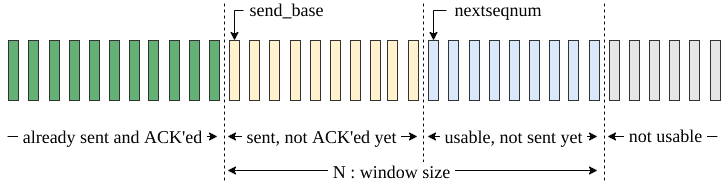
\includegraphics[width=1\linewidth]{./images/gobackn.png}
\end{figure}
Ogni volta che il primo frame della finestra viene mandato, questa "scorre" di un frame verso quelli ancora da mandare. Individuiamo quattro insiemi disgiunti di frame:
\begin{itemize}
	\item I frame mandati non confermati (ACKed, prima parte della finestra).
	\item I frame non mandati ma utilizzabili (seconda parte della finestra).
	\item Prima della finestra, abbiamo i frame mandati e confermati.
	\item Dopo la finestra, i frame non utilizzabili.
\end{itemize}

\subsubsection{Receiver}
Riceve i pacchetti e risponde con gli \verb|ACK| rispettivi. Quando non riceve il pacchetto giusto\footnote{Un esempio di pacchetto non corretto? Il pacchetto con numero di sequenza 3 dopo aver ricevuto il pacchetto 1 è sbagliato: manca il pacchetto 2.}, scarta il pacchetto, manda un duplicato dell'ultimo \verb|ACK| ricevuto correttamente.

\begin{figure}[htp]
	\centering
	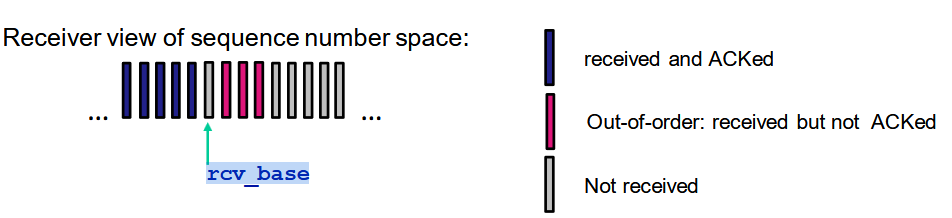
\includegraphics[width=1\linewidth]{./images/gobackn2.png}
\end{figure}


\subsubsection{Criticità del Go-Back-N}
Osserviamo che se l'$n$-esimo pacchetto non è stato ricevuto con successo, tutti i successivi pacchetti mandati verranno scartati. Nell'immagine della prossima pagina, si evidenzia come il primo inoltro dei pacchetti 3, 4 e 5 sia praticamente cestinato. È un algoritmo solido e reliable, ma rischia grosse perdite di tempo a causa dell'\verb|ACK| cumulativo.
\newpage

\begin{figure}[htp]
	\centering
	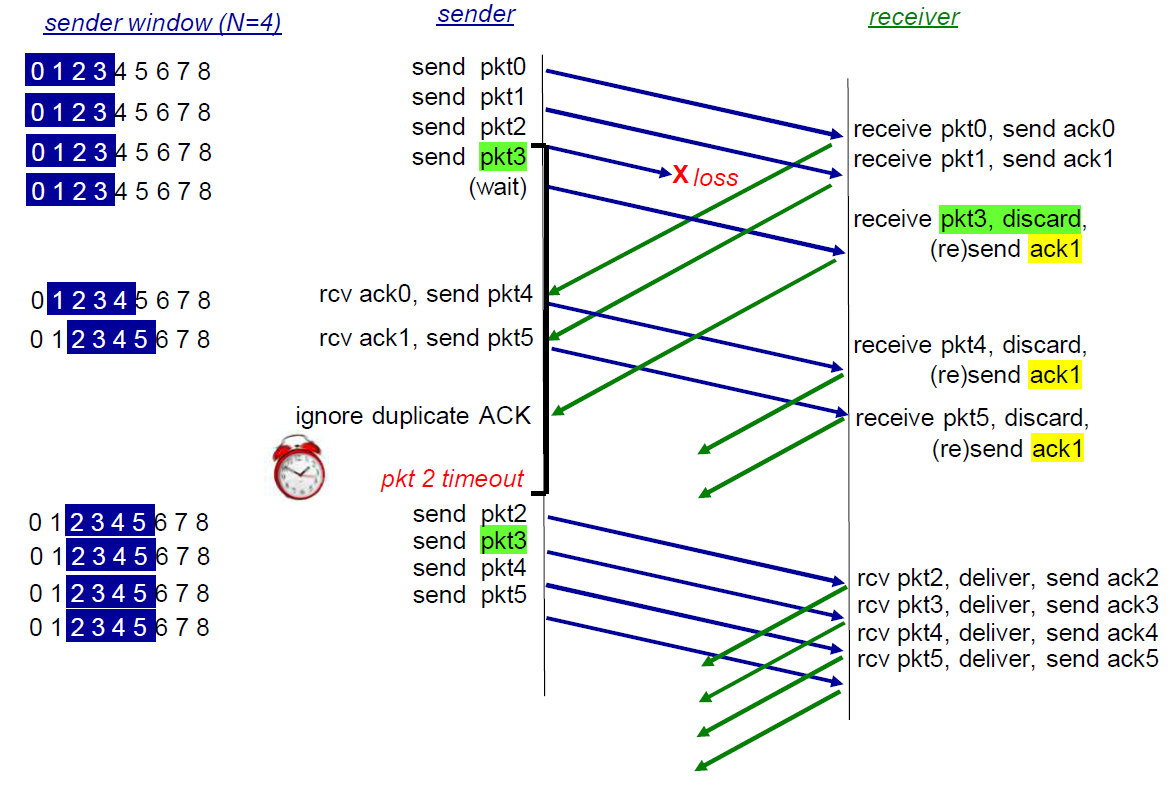
\includegraphics[width=1\linewidth]{./images/gobacknn.png}
	\caption{Go-back-n.}
\end{figure}

\newpage

\subsection{Algoritmi per la pipeline - Selective Repeat}
Col selective repeat, i frame che si perderebbero durante il time-out, sono bufferizzati in una memoria all'interno del dispositivo (in una look-up-table), in modo da velocizzarne il caricamento e non dover richiede il reinvio dal sender. Gli ACK dei pacchetti ricevuti correttamente vengono rimandati regolarmente. 

\begin{figure}[htp]
	\centering
	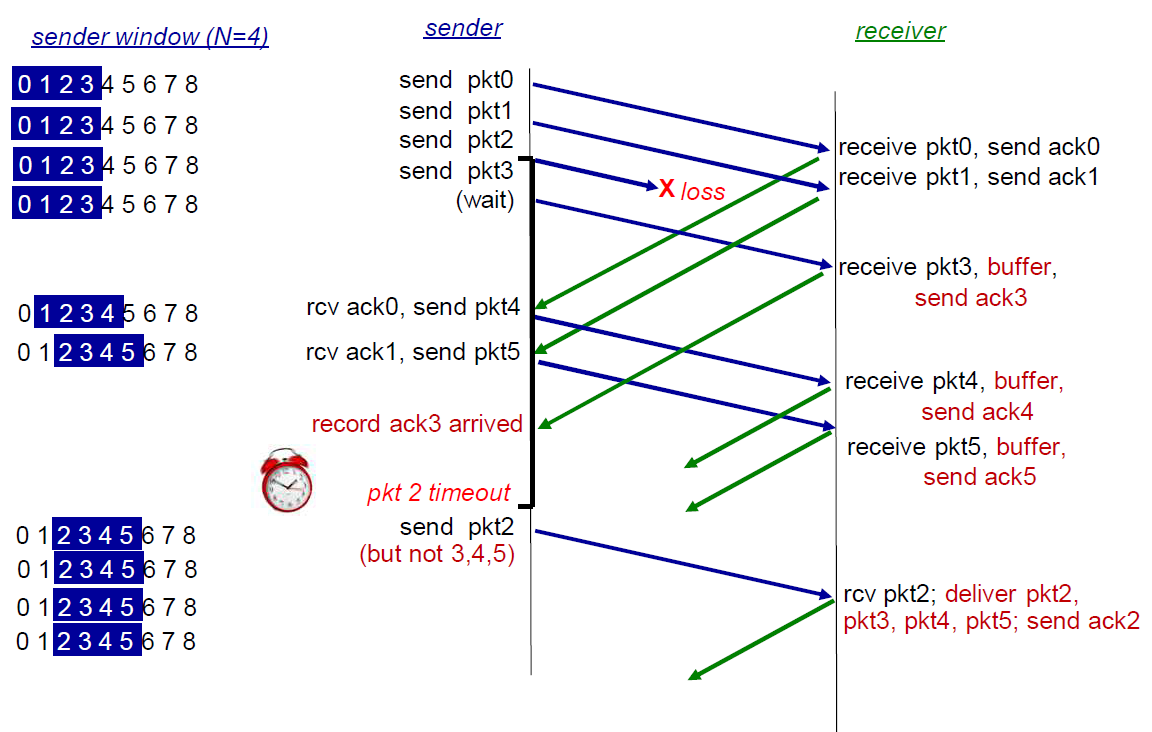
\includegraphics[width=0.75\linewidth]{./images/selectiverepeat.png}
\end{figure}

\subsubsection{Sender}
\begin{itemize}
	\item Trasmette fino a $n$ pacchetti \textbf{senza attendere ACK}.
	\item Ogni pacchetto ha un \textbf{timer personale} per la ritrasmissione.
	\item Ricevuto l'ACK dell'$n$-esimo pacchetto, viene \textbf{marcato come ricevuto}.
	\item Il primo frame della windows è sempre il primo frame della sequenza non ancora confermato.
\end{itemize}
\subsubsection{Receiver}
\begin{itemize}
	\item \textbf{I pacchetti non ricevuti in ordine vengono inseriti in un buffer}.
	\item A ogni pacchetto ricevuto, consegue l'invio di un \textbf{ACK}.
	\item Se l'$n$-esimo pacchetto viene ricevuto, e ci sono \textbf{pacchetti subito successivi bufferizzati}, questi vengono \textbf{passati al layer superiore}.
	\item Il receiver potrebbe ricevere un pacchetto con \textbf{numero di sequenza precedente alla finestra}: in tal caso, \textbf{reinvierà l'ACK}.
\end{itemize}

\subsubsection{Pro del Selective Repeat}
\textbf{Meno ritrasmissioni inutili}, maggiore efficienza in canali con alta perdita di pacchetti.
\subsubsection{Contro del Selective Repeat}
\begin{itemize}
	\item Il buffer non ha \textbf{memoria infinita}, potrebbe saturarsi.
	
	\item Possono esserci \textbf{ambiguità} causati dai \textbf{codici sequenza ripetuti}. Per non incorrere in questi problemi, deve essere rispettata la seguente disequazione:
	$$
	\text{K-seq (Numero max sequenza)} \geq 2 \cdot \text{Window Size}
	$$
	
	\begin{figure}[htp]
		\centering
		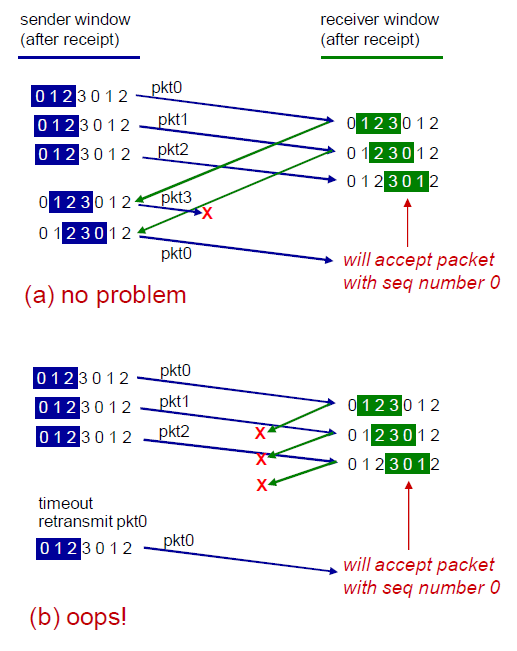
\includegraphics[width=0.75\linewidth]{./images/selectiverepeat3.png}
		\caption{Ambiguità dei codici sequenza nel Selective Repeat}
	\end{figure}
\end{itemize}

\newpage

\section{TCP}
Sta per \textbf{Transmission Control Protocol}. Assieme a UDP, è il \textbf{protocollo del layer di trasporto più importante}. Sfruttato da tantissime applicazioni del layer superiore, offre un trasporto affidabile, basato sui meccanismi della modello RDT 3.0.  Tra le sue funzionalità, offre:

\begin{itemize}
	\item \textbf{Addressing} / \textbf{multiplexing}.
	\item Stabilimento, gestione e terminazione della \textbf{connessione}.
	\item \textbf{Data Handling} e impacchettamento.
	\item \textbf{Trasferimento dei dati} (banalmente).
	\item Fornisce \textbf{specifiche} relative alla reliability della rete.
	\item \textbf{Controllo del flusso} e gestione della \textbf{congestione}.
\end{itemize}

\subsubsection{Cosa non fornisce il TCP?}
\begin{itemize}
	\item Non garantisce \textbf{sicurezza}.\\
	È \textbf{vulnerabile} ad hacking, attacchi man-in-the-middle, sniffing e simili.
	\item Non da \textbf{specifiche sull'application layer}.\\
	Non fa ipotesi sui layer superiori (ed è giusto che sia così! Altrimenti le applicazioni si dovrebbero adattare alle ipotesi fatte da TCP).
	\item Non mantiene i \textbf{message boundaries}.\\
	Non stabilisce i confini dei messaggi. Sono i protocolli del layer applicativo che stabiliscono come interpretare i messaggi e ricostruire i dati, tramite caratteri di terminazione, lunghezze prestabilite o header.
	
	\item Non da \textbf{garanzie sul throughput}.
	
	\item \textbf{Non supporta trasferimento multicast}, ossia trasferimento da un mittente a molti destinatari in una sola operazione.
\end{itemize}

\newpage

\subsection{TCP-State Model}
È un diagramma degli stati che descrive le fasi di una connessione TCP.
\begin{figure}[htp]
	\centering
	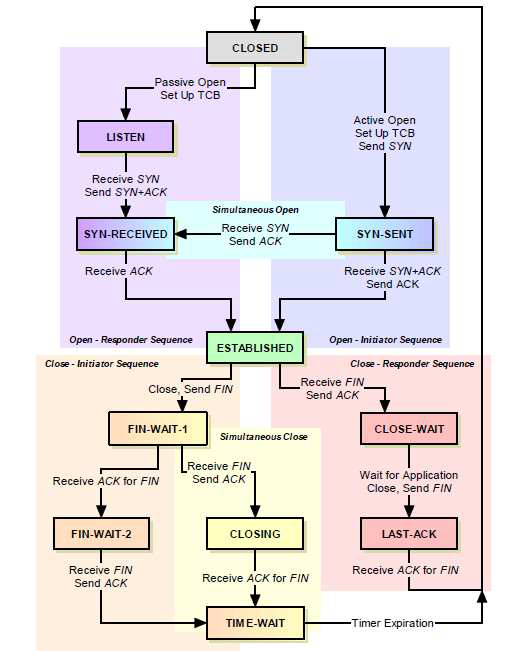
\includegraphics[width=0.7\linewidth]{./images/TCPSTATEMACHINE.png}
\end{figure}
\subsection{Fasi di apertura della connessione (3-way-handshake)}
\begin{enumerate}
	\item CLOSED.
	\begin{enumerate}
		\item Stato iniziale, nessuna connessione attiva.
		\item Un'applicazione può avviare una connessione o attenderne una in ingresso.
	\end{enumerate}
	\item LISTEN (solo lato server).
	\begin{enumerate}
		\item Il server è in ascolto, pronto a ricevere connessioni (passive open).
		\item Se riceve un segmento \verb|SYN|, risponde con \verb|SYN-ACK| e passa allo stato \verb|SYN|
	\end{enumerate}
	\item SYN-SENT (solo lato client).
	\begin{enumerate}
		\item Il client avvia una connessione inviando un segmento \verb|SYN|
		\item Se riceve \verb|SYN+ACK| risponde con \verb|ACK| e la connessione è stabilita (passando a \verb|ESTABLISHED|)
	\end{enumerate}
	\item SYN-RECEIVED
	\begin{enumerate}
		\item Il server ha ricevuto \verb|SYN| e inviato il \verb|SYN-ACK|
		\item Quando riceve l'\verb|ACK| finale dal client, la connessione è stabilita (\verb|ESTABLISHED|).
	\end{enumerate}
	\item ESTABLISHED
	\begin{enumerate}
		\item Stato operativo della connessione in cui i dati vengono trasmessi tra client e server.
		\item La connessione si trova in questo stato finché non viene chiusa.
	\end{enumerate}
	\subsection{Fasi della chiusura della connessione (4-way-handshake)}
	\item FIN-WAIT-1.
	\begin{enumerate}
		\item Il lato che inizia la chiusura invia un segmento \verb|FIN|.
		\item Attende un \verb|ACK| per il \verb|FIN| o un \verb|FIN| dall'altro lato.
	\end{enumerate}
	\item CLOSE-WAIT.
	\begin{enumerate}
		\item Il lato che riceve il \verb|FIN| invia un \verb|ACK| e passa in \verb|CLOSE-WAIT|.
		\item Aspetta che l'applicazione chiuda il socket, poi invia un \verb|FIN|.
	\end{enumerate}
	\item FIN-WAIT-2
	\begin{enumerate}
		\item Il lato che ha inviato il primo \verb|FIN| ha ricevuto un \verb|ACK| ed è in attesa del \verb|FIN| dell'altro lato
	\end{enumerate}
	
	\item LAST-ACK.
	\begin{enumerate}
		\item Il lato che ha ricevuto il \verb|FIN| deve terminare, invia un \verb|FIN| e attende un \verb|ACK|.
	\end{enumerate}
	
	\item TIME-WAIT
	\begin{enumerate}
		\item Dopo aver ricevuto l'ultimo \verb|ACK|, il lato iniziatore della chiusura entra in \verb|TIME-WAIT| per un certo tempo (solitamente il doppio del Maximum Segment Timeline).\\
		Questo assicura che l'altro lato abbia ricevuto l'ACK finale prima di tornare a \verb|CLOSED|.
	\end{enumerate}
	
	\item CLOSING
	\begin{enumerate}
		\item Caso raro in cui entrambi i lati inviano un \verb|FIN| contemporaneamente.
		\item Entrambi inviano e ricevono un \verb|ACK|, poi passano a \verb|TIME-WAIT|.
	\end{enumerate}
\end{enumerate}
\newpage

\subsection{Struttura dei segmenti del TCP}
Gli header dei segmenti TCP occupano \textbf{dai 20 ai 60 byte}, (ricordiamo che gli header UDP occupano solo 8 byte). 

\begin{figure}[htp]
	\centering
	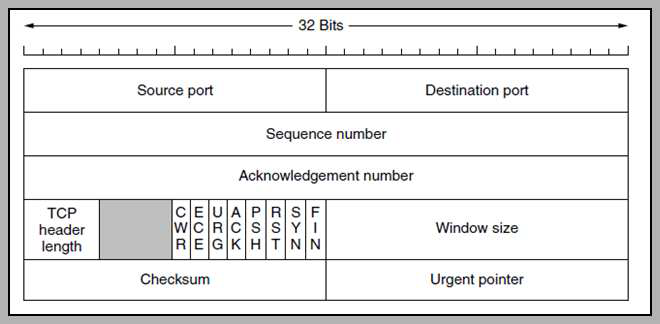
\includegraphics[width=0.8\linewidth]{./images/SEGMENTCP.png}
\end{figure}

\begin{itemize}
	\item \textbf{Source port} e \textbf{Destination port} indicano le porte dei processi del sender e receiver associati alla connessione TCP.  16 bit ciascuno.
	
	\item \textbf{Sequence number}. \\
	Viene incrementato di $n$ ogni volta che $n$ byte sono trasmessi. Mandato un pacchetto TCP di \\1400 byte, il prossimo valore sarà il precedente numero di sequenza + 1400. 32 bit.
	
	\item \textbf{Acknowledgment number}.\\
	Se \verb|ACK| è abilitato, ritorna il sequence number del prossimo pacchetto che si aspetta di ricevere. \\
	32 bit.
	
	\begin{Verbatim}
		CLIENT                  SERVER
		#seq = 1
		Len = 669     -->
		<--       ACK (669 + 1 =) 670
		#seq = 670
		Len = 1460    -->
		<--       ACK (670 + 1460 =) 2130
		#seq = 2130
		Len = 1460    -->
		<--       ACK 3590
		[...] 
		END OF TCP CONNECTION
	\end{Verbatim}
	
	
	Notiamo che \textbf{il protocollo TCP è full-duplex}: gli host ricevono e mandano dati nella stessa connessione.
	
	\item \textbf{TCP header length} o \textbf{Data Offset}.\\
	Specifica il numero di double word (4 byte) dell'header del segmento TCP. 4 bit. 
	\item Dello spazio libero per sviluppi futuri del protocollo. 4 bits.
	
	\item \textbf{8 flags}, un bit per flag.
	\begin{itemize}
		\item \verb|CWR| Congestion Window Reduced.\\ 
		A 1 indica che l'host sorgente ha ricevuto un segmento TCP con il flag ECE impostato a 1.
		\item \verb|ECE| Explicit Congestion Notification-Echo.\\ 
		A 1 indica che l'host supporta ECN durante il 3-way handshak
		\item \verb|URG|.\\
		A 1 indica che nel flusso sono presenti dati urgenti specificati nel campo urgent pointer.
		\item \verb|ACK|.\\
		A indica che il campo Acknowledgment number è valido.
		\item \verb|PSH|.\\
		A 1 indica che i dati in arrivo non devono essere bufferizzati ma passati subito ai livelli superiori dell'applicazione.
		\item \verb|RST|.\\
		A 1 indica che la connessione non è valida; viene utilizzato in caso di grave errore; a volte utilizzato insieme al flag ACK per la chiusura di una connessione.
		\item \verb|SYN|.\\
		A 1 indica che il mittente del segmento vuole aprire una connessione TCP con l'host destinatario e specifica nel campo Sequence number il valore dell'Initial Sequence Number (ISN); questo sincronizza i numeri di sequenza dei due host. L'host che ha inviato il SYN deve attendere dall'host remoto un pacchetto SYN/ACK.
		\item \verb|FIN|.\\
		A 1 indica che l'host mittente del segmento vuole chiudere la connessione TCP. Il mittente attende la conferma dal ricevente (con un FIN-ACK). La connessione sarà ancora chiusa per metà: l'host che ha inviato FIN non potrà più inviare dati, mentre l'altro host ha il canale di comunicazione ancora disponibile. L'altro host dovrà inviare il pacchetto con FIN impostato. Dopo il relativo FIN-ACK, la connessione sarà considerata completamente chiusa.
	\end{itemize}
	
	\item \textbf{Window size}.\\ 
	Indica la dimensione della finestra di ricezione del mittente. 16 bit.
	
	\item \textbf{Checksum}.\\
	Serve a verificare la validità del segmento. 16 bit.
	
	\item \textbf{Urgent pointer}.\\
	Punta a un dato urgente, ma solo se \verb|URG |=1. Indica l'offset in byte dal sequence number ai dati urgenti all'interno del flusso. 16 bit.
	
	\item Sotto troveremo anche dei byte dedicati ad ulteriore possibili \textbf{impostazioni}, e, chiaramente, lo spazio dedicato ai \textbf{dati da inviare}.
\end{itemize}


\newpage

\section{Migliorare il Througput - MMS e MTU}
I meccanismi appena esposti rendono TCP un protocollo affidabile. Tuttavia, anche il \textbf{throughput} è un fattore da tenere in considerazione. Per massimizzare il throughput, dobbiamo analizzare una serie di parametri.

\subsection{MMS, MTU}
\begin{itemize}
	\item \textbf{MMS - Maximum Segment Size}.\\
	Indica la dimensione massima dei dati che possono essere inviati in un singolo segmento TCP (esclusi gli header TCP/IP). Questo valore viene solitamente scelto in virtù dal frame più grande che il sender può trasmettere. 
	
	\item \textbf{MTU - Maximum Transmission Unit}.
	$$\text{MSS} + \text{dimensione dell'header TCP + dimensione dell'header IP}$$
	
\end{itemize}

Il protocollo TCP richiede un MTU minimo di 576 bytes, e quindi un MSS minimo di 536 bytes + 40 bytes di header IP (20 byte) e TCP (20 bytes).

\section{Migliorare il Througput - Retransmission Time-Out}
Affrontando l'argomento del \textbf{Reliable Data Transfer}, abbiamo spiegato che il meccanismo di \textbf{temporizzazione è fondamentale} per ottenere un trasferimento dati \textbf{reliable}. Nonostante ciò, bisogna trovare un buon \textbf{compromesso} per non impattare negativamente sul througput. \textbf{Il time-out va stabilito in funzione del Round Trip Time}.

\begin{itemize}
	\item \textbf{Time-out troppo lungo?}\\
	Reazione troppo lenta alla perdita dei pacchetti. Conseguenza di un time-out di molto maggiore dell'RTT.
	
	\item \textbf{Time-out troppo corto?}\\
	Gli ACK potrebbero non arrivare in tempo, richiedendo ritrasmissioni non necessarie. Time-out quanto o poco più lungo dell'RTT.
\end{itemize}

Per decidere il tempo opportuno per il time-out, bisogna avere una stima \footnote{Il round trip time è un valore misurabile, ma variabile. L'obiettivo che ci poniamo è stimare sempre il prossimo valore dell'RTT in funzione dei precedenti. Ricordiamo inoltre che ping permette di ottenere il Round Trip Time con un server.} valida dell'RTT. 


\subsection{Stimare il Round Trip Time}
Il Sample\_RTT è la misura del tempo di trasmissione di un segmento. La misura avviene dall'invio del segmento fino alla ricezione dell'ACK.\\
Un algoritmo che potrebbe essere utilizzato per stimare il time-out è quello di \textbf{Karn}: questo tuttavia, non tiene conto di possibili ritrasmissioni dei pacchetti non-acknowledged, che nella realtà avvengono molto spesso.\\
Utilizzeremo quindi una \textbf{media pesata} chiamata \textbf{Exponential Weighted Moving Average}.

\newpage

\subsection{Exponential Weighted Moving Average - EWMA}
Il peso, ovvero l'influenza dei campioni passati sulla media calcolata decresce in maniera esponenziale.

$$
\text{Estimated\_RTT}_n = (1-\alpha)\cdot \text{Estimated\_RTT}_{n-1} + \alpha \cdot  \text{Sample\_RTT}_n
$$

Dove il $\text{Sample\_RTT}_n$ è l'$n$-esima misurazione. Il valore $\alpha$ è detto \textbf{weighted value}, e stabilisce il peso dell'ultima misura rispetto a quello dell'ultima stima sulla media. Un valore tipico è $\alpha = \frac{1}{8} = 0,125$. Il valore di $\alpha$ varia, non è raro l'utilizzo di tecnica try and error per trovare il valore che permette di ottenere stime ottime.
Euristiche varie e tecnologie AI sono utilizzate per ottenere stime via via più accurate.

\begin{figure}[htp]
	\centering
	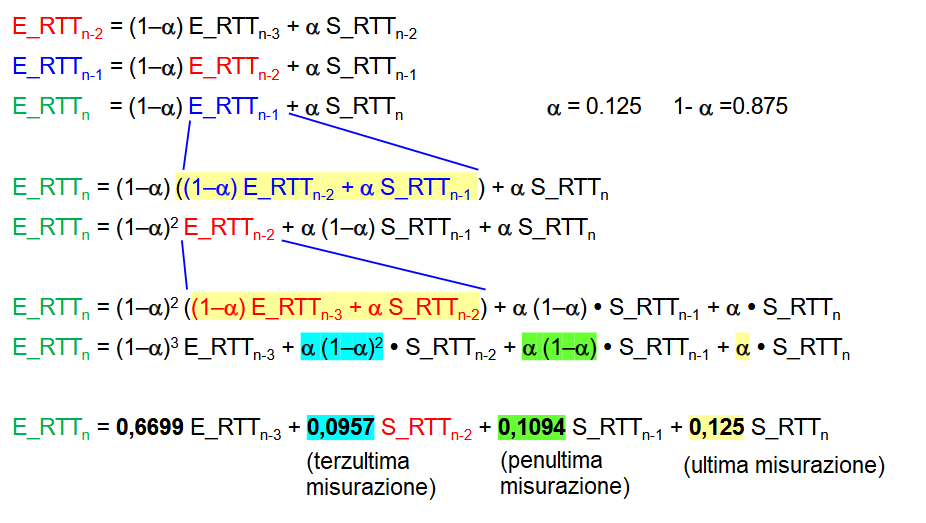
\includegraphics[width=1\linewidth]{./images/rtt.png}
\end{figure}

\subsection{Deviazione del RTT}
La natura variabile dell'RTT ci porta a voler tener conto anche del valore della deviazione standard.
$$
\text{Dev\_RTT} = (1-\beta) \cdot \text{Dev\_RTT} + \beta \cdot |\text{Sample\_RTT} - \text{Estimated\_RTT} |
$$
Un valore tipico è $\beta = \frac{1}{4}= 0.25$. 
\subsection{Risultato finale - Retransmission Time-out}

Dati alla mano, possiamo finalmente stabilire l'RTO, ovvero il valore da dare al timer.

$$
\text{Retransmission Time-Out} = \text{Estimated\_RTT} + 4 \cdot \text{Dev\_RTT}
$$
Con un valore di partenza pari a un secondo (RFC 6298).

\newpage

\section{Timer}
Nonostante RDT stabilisca che ad un pacchetto venga associato un timer, TCP riduce la complessità di gestione gestendo esclusivamente un timer alla volta. Dopo la ricezione dell'ACK dell'$n$-esimo pacchetto, il timer per il segmento $n+1$ non ancora acknowledged viene avviato.

\subsection{Fast-Retransmit}
Per ridurre il tempo di attesa dato dal time-out, si include un'altra condizione per le ritrasmissioni. Questo meccanismo è detto fast retransmit:
se il sender manda tre ACK consecutivi per lo stesso pacchetto mancante (ovvero l'ACK dell'ultimo pacchetto consegnato con successo), viene attivata istantaneamente la ritrasmissione del pacchetto.

\begin{figure}[htp]
	\centering
	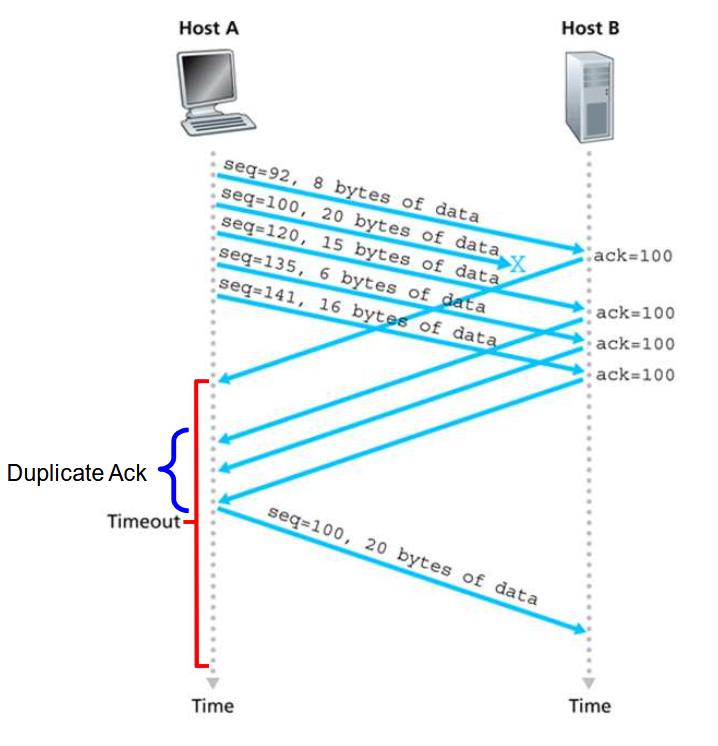
\includegraphics[width=1\linewidth]{./images/fastretransmission.png}
\end{figure}


Questo meccanismo si basa sulla considerazione che, dopo il terzo ACK relativo allo stesso pacchetto non pervenuto, è probabile che questo si sia perso, e vada ritrasmesso. 

\newpage

\section{TCP - Controllo di flusso}
Il problema del produttore-consumatore si ripresenta anche qui: se il Network Layer fornisce dati al buffer del layer di trasporto ad una velocità superiore rispetto a quella con cui l'applicazione può toglierli dal buffer, si corre il rischio di saturarlo.\textbf{ Gestire in maniera consona il flusso è fondamentale} per evitare di dover scartare pacchetti, ed il protocollo TCP implementa dei meccanismi con questo scopo. \textbf{UDP non ha meccanismi equivalenti}.


\subsection{Finestra di ricezione}
Il controllo del flusso viene gestito tramite una variabile chiamata \textbf{Receive Window}, \verb|rwnd|, che specifica al mittente lo spazio libero nel buffer di ricezione del destinatario. Il valore \verb|rwnd| viene aggiornato e trasmesso al mittente tramite un campo dell'header TCP degli ACK.

Quando viene instaurata una connessione TCP, il destinatario riserva un buffer di ricezione denominato \verb|RcvBuffer|, di cui la dimensione può essere configurata tramite le opzioni del socket.

$$
\text{rwnd} = \text{ReceiverBufferSize} - (\text{LastByteReceived} - \text{LastByteRead})
$$

Dove 
\begin{itemize}
	\item \textbf{LastByteReceived} è il numero dell'ultimo byte ricevuto dal livello di rete e inserito nel buffer.
	\item \textbf{LastByteRead} è il numero dell'ultimo byte letto dal buffer dall'application layer.
\end{itemize}

\subsubsection{Circostanza problematica}
Quando il buffer del destinatario si riempie completamente, il receiver manda $\text{rwnd}= 0$, il sender si blocca. Da qui in poi, sia sender che receiver si bloccheranno: come fa il receiver ad aggiornare il sender senza ACK da mandare?
Per risolvere questo problema, il protocollo TCP impone un meccanismo in cui il sender invia dei \textbf{probe packets} contenenti un singolo byte di dati forzando una risposta dal ricevente.

\subsection{Algoritmo di Nagle}
L‘algoritmo di Nagle è una tecnica utilizzata nei protocolli di trasporto, in particolare nel protocollo TCP, per ridurre l‘overhead generato dall‘invio di piccoli pacchetti (ricordiamo che l'RTT è un tempo che viene atteso ad ogni trasmissione di dati). 
Questo è particolarmente utile nelle applicazioni che generano molte trasmissioni di dati di piccole dimensioni, come Telnet, che invia pacchetti di dimensioni minime (tipicamente di 1 byte).
L'obiettivo è \textbf{aggregare dati di piccole dimensioni} nel buffer di trasmissione, \textbf{per inserirli in pacchetti più grandi quando l'RTT della rete è alto}.

\subsubsection{Algoritmo}
\begin{enumerate}
	\item Verificare se ci sono dati tra trasmettere. Se sì, step 2, altrimenti step 3.
	\item Verificare se $\verb|rwnd| \geq MSS$ e che i dati siano $\geq MSS$. Se sì, step 5, altrimenti step 3.
	\item Verifica se stai aspettando un ACK. Se sì, step 4, altrimenti 5.
	\item Accoda i dati da mandare fino alla ricezione dell'ACK, vai a step 5.
	\item Manda i dati, end.
\end{enumerate}

\subsubsection{Pseudocodice}
\begin{verbatim}
	if available_data > 0:
	if window_size >= MSS AND available_data >= MSS:
	send_a_MSS_segment
	else:
	if waiting_for_an_ack == true:
	enqueue_data_in_buffer    /* until an acknowledge is received */
	else:
	send_data
\end{verbatim}

In programmi che richiedono bassa latenza e alta reattività, alcuni sistemi operativi possono disabilitare questo algoritmo tramite l'opzione \verb|TCP_NODELAY| nel socket API.


\section{Connessione TCP}
Il three-way handshake è tra gli aspetti caratterizzanti del protocollo TCP. Andiamo adesso ad analizzarlo nel dettaglio, e ad analizzare perché un two-way handshake non sarebbe funzionale.

\subsection{2-way handshake (un'intuizione inconcludente)}
Prima dell'introduzione del three-way handshake, si è considerato un approccio più semplice (e vicino a quello umano) con un \textbf{two-way handshake}. Si è presto realizzato che un two-way handshake apre le porte a situazioni di \textbf{connessioni half open}. 

\begin{enumerate}
	\item $A$ richiede la connessione a $B$.
	\item $B$ manda un'ACK, apre la connessione
	\item $A$ riceve l'ACK, partecipa alla connessione.
\end{enumerate}
\textbf{E se l'ACK si perde?}

\begin{enumerate}
	\item $A$ chiede la connessione a $B$.
	\item $B$ manda un'ACK e apre la connessione.
	\item L'ACK si perde o il client $A$ crasha. La connessione del server $B$ rimane aperta e in attesa.
\end{enumerate}

Il server $B$ entrerà nello stato \verb|ESTABLISHED|, il client $A$ invece no. Si ottiene quindi una connessione half-open anomala e inutilizzabile.

\subsection{3-way handshake}

Il three-way handshake gestisce queste circostanze tramite un flag \verb|RST| che può essere messo a 1 in un segmento TCP. 

\begin{figure}[htp]
	\centering
	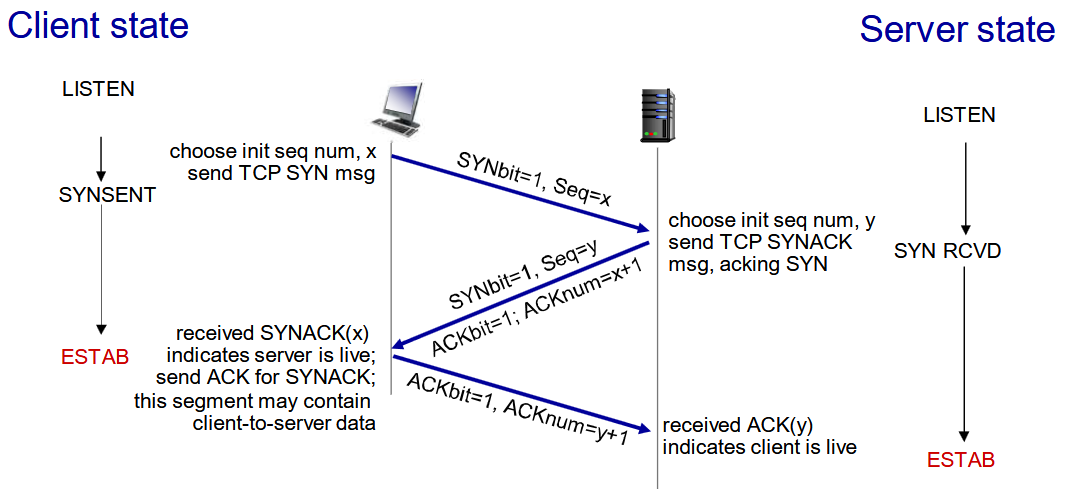
\includegraphics[width=1\linewidth]{./images/3wayhandshake.png}
\end{figure}

\begin{figure}[htp]
	\centering
	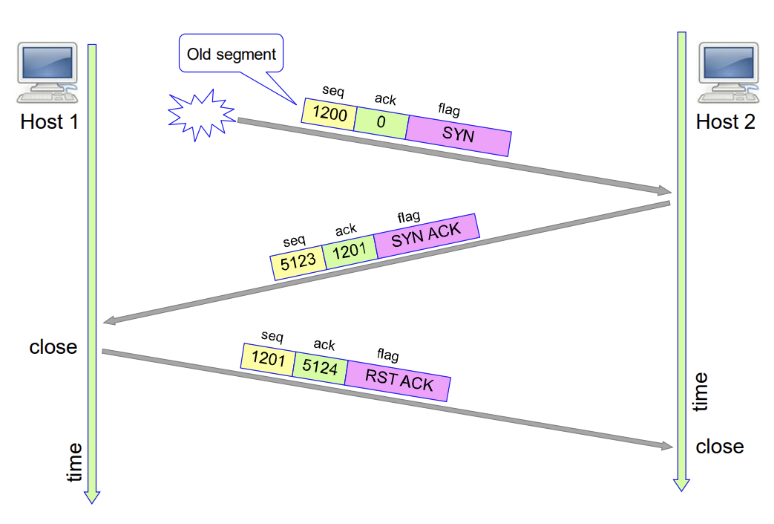
\includegraphics[width=0.75\linewidth]{./images/rstack.png}
\end{figure}


Se l'host $A$ riceve un segmento TCP che \textbf{non riconosce} (e quindi da una connessione che non è stata stabilita con successo, presumibilmente half-open), questo manderà un segmento TCP di \verb|RST ACK| con \verb|RST|=1 per chiedere l'interruzione immediata di questa presunta mezza connessione.

\newpage

\subsection{4-way handshake (2*2-way handshake) per chiusura connessioni}
\underline{La chiusura delle connessioni TCP avviene tramite due 2-way handshake.}\footnote{Si è deciso di sottolineare questa parte in quanto è una puntalizzazione molto importante, soprattutto in sede d'esame.} 
\begin{enumerate}
	\item Il client termina l'invio dei dati: invia segmento con flag \verb|FIN|.
	\item Il server risponde con \verb|ACK|.
	\item Il server è pronto a chiudere la connessione: invia segmento con flag \verb|FIN|.
	\item Il client risponde con \verb|ACK|, chiudendo definitivamente la connessione.
\end{enumerate}
\begin{figure}[htp]
	\centering
	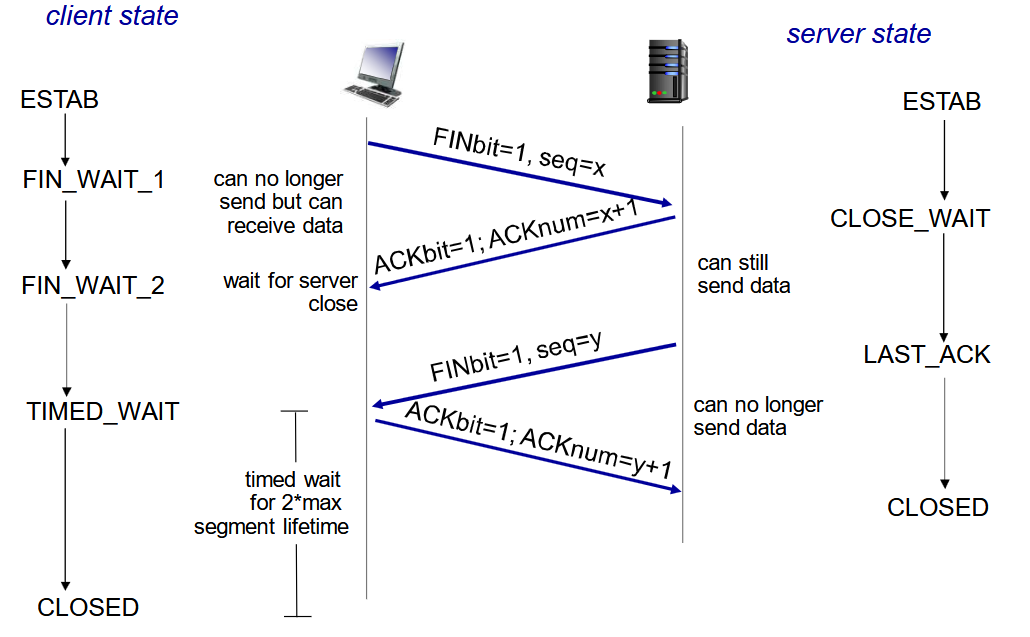
\includegraphics[width=1\linewidth]{./images/4wayhandshake.png}
\end{figure}

Osserviamo che dopo l'invio dell'ultimo \verb|FIN-ACK|, si avvierà un timer \textbf{TIME-WAIT} di tempo pari a 
2 volte tempo di vita massimo di un segmento: ciò darà il tempo ai pacchetti residui nella rete di arrivare (o di far scadere il loro timer) per evitare che vengano ricevuti a connessione ormai chiusa.

\newpage

\section{Controllo della congestione}
La \textbf{gestione delle trasmissioni} è fondamentale per evitare non solo di sovraccaricare i receiver (eventualità gestita tramite il \textbf{controllo del flusso}), ma anche per evitare il sovraccarico della rete, con conseguente congestione.
Il protocollo TCP gode di meccanismi per gestire la congestione, per ridurre la velocità di trasmissione e minimizzare i danni della congestione.

\subsection{Scenario 1 - due mittenti e receiver, router con buffer illimitato}
Nell'analisi della congestione di rete, è importante conoscere dei valori, quali


\begin{itemize}
	\item $\lambda_{\verb|in|}$, frequenza media di invio (dai mittenti).
	\item $\lambda_{\verb|out|}$, la frequenza di arrivo di byte al ricevente.
	\item $R$, la capacità del collegamento condiviso.
\end{itemize}
Quando $\lambda_{\verb|in|}\geq\lambda_{\verb|out|}$, inizia a crearsi congestione.\\
Consideriamo due host mittenti $A$ e
$B$ che inviano a due host destinatari attraverso un router intermedio, e supponiamo che il suo buffer sia illimitato.

\begin{figure}[htp]
	\centering
	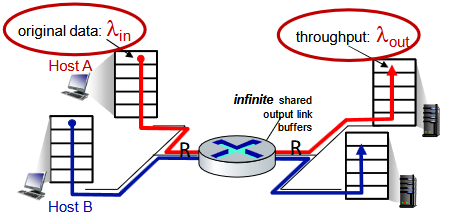
\includegraphics[width=0.5\linewidth]{./images/bufferillimitato.png}
\end{figure}

\begin{itemize}
	\item Se $\lambda_{\verb|in|}\leq \frac{R}{2}$, il router riesce ad inoltrare i pacchetti senza ritardi significativi, e $\lambda_{\verb|out|}=\lambda_{\verb|in|}$. Dividiamo $R$ in due perché abbiamo due host che mandano.
	
	\item Se $\lambda_{\verb|in|} $ aumenta fino a $\frac{R}{2}$, il $\lambda_{\verb|out|}$ massimo si stabilizza su $\frac{R}{2}$.
	
	\item Se $\lambda_{\verb|in|} > \frac{R}{2}$, il throughput non aumenta, ma il numero di pacchetti accodati nel buffer del router cresce senza limite, aumentando il ritardo medio di trasmissione.
\end{itemize}

\newpage

\subsection{Scenario 2 - due mittenti e receiver, un router con buffer limitato}
Quando il buffer di un router è pieno, pacchetti vengono scartati. Di fronte a circostanze simili, TCP prevede ritrasmissione, con conseguente aumento della latenza complessiva aumenta e riduzione frequenza media di invio $\lambda_{\verb|in|}$ diminuisce, in quanto vengono rimandati gli stessi pacchetti. $\lambda_{\verb|in|}'$ tiene conto sia dei dati originali, che delle ritrasmissioni. Distinguiamo ora dei casi di quest scenario.

\begin{enumerate}
	\item \textbf{Nessuna perdita di pacchetti - Perfect Knowledge.}\\
	Se i sender fossero in grado di determinare in anticipo se il router ha spazio disponibile nel buffer, invierebbe un pacchetto solo quando può essere immediatamente elaborato, ottenendo $\lambda_{\verb|in|} = \lambda_{\verb|in|}'$, $\lambda_{\verb|out|}=\lambda_{\verb|in|} \leq \frac{R}{2}$ e zero latenza (perlomeno, causata dal router).
	
	\item \textbf{Ritrasmissione solo per pacchetti persi - Some perfect Knowledge.}\\
	I sender non conoscono lo stato del buffer, e ritrasmettono un pacchetto solo quando hanno la certezza che sia stato perso. Supponendo che $\lambda_{\verb|in|}'=\frac{R}{2}$, $\lambda_{\verb|out|} < \frac{R}{2}$ a causa delle ritrasmissioni.
	
	\item \textbf{Caso reale - duplicati non necessari}.\\
	I sender non conoscono lo stato del buffer, e potrebbero avere un \textbf{timer di ritrasmissione troppo breve}. Questo implica un utilizzo innecessario del buffer del router, della banda e delle risorse di elaborazione. Questo potrebbe addirittura portare ad un throughput di circa $\lambda_{\verb|out|}=\frac{R}{4}$.
\end{enumerate}

\begin{figure}[htp]
	\centering
	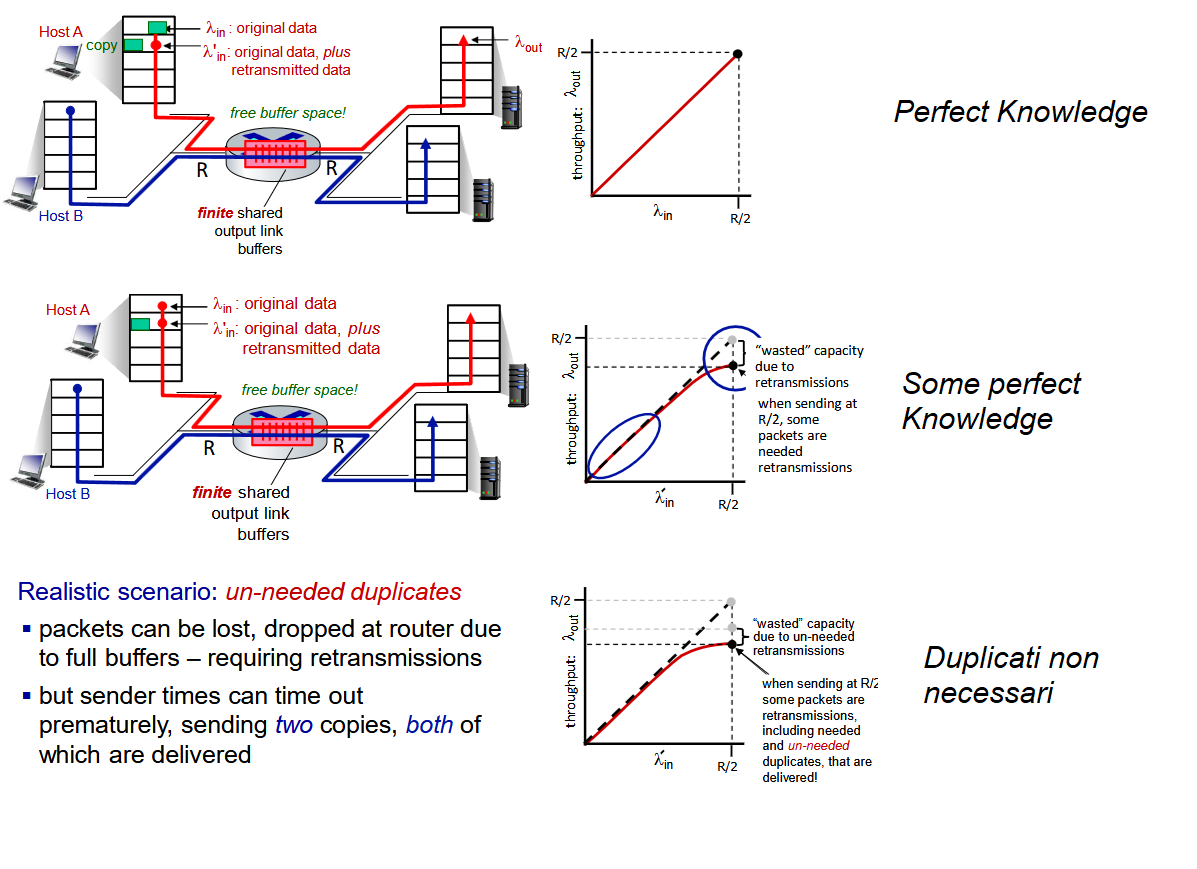
\includegraphics[width=1\linewidth]{./images/limitedbuffer.png}
\end{figure}


\newpage

\subsection{Terzo scenario - quattro mittenti, più router limitati e percorsi}
In questo scenario, quattro mittenti inviano pacchetti su percorsi composti da più collegamenti, condividendo router intermedi. Ogni host utilizza un meccanismo di ritrasmissione basato su timeout, e la rete ha buffer di dimensione finita.

\begin{figure}[htp]
	\centering
	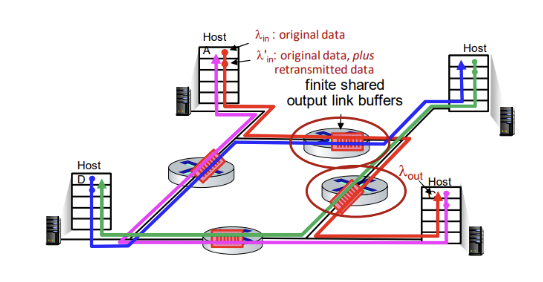
\includegraphics[width=1\linewidth]{./images/4mittentiblahblah.png}
\end{figure}

Abbiamo quattro sender che inviano pacchetti in quattro percorsi con più router, e quindi più possibili percorsi. Ogni router trasmette a capacità $R$. A valori di $\lambda_{\verb|in|}$ piccoli, $\lambda_{\verb|in|} = \lambda_{\verb|in|}'$, non si hanno overflow dei buffer e nemmeno ritrasmissioni. Al crescere del valore di $\lambda_{\verb|in|}$, inizia il rischio di ritrasmissioni, per cui $\lambda_{\verb|in|}' > \lambda_{\verb|in|}$.

\newpage

\section{Meccanismi per gestire la congestione}
Abbiamo quindi capito che la congestione è un fenomeno che si riscontra quando \textbf{il traffico si avvicina o supera la capacità della rete} $R$. Per limitarlo, si opera sulla finestra di trasmissione degli host \verb|cwnd|, aumentando e riducendo in maniera opportuna il numero di pacchetti consentiti contemporaneamente sulla rete (senza aver ricevuto un ACK).
\subsection{Due approcci}
\begin{itemize}
	\item \textbf{Approccio Network-assisted.}\\
	I router forniscono un \textbf{feedback diretto} agli host sender e receiver (di un flusso passante lo stesso router) in merito alla congestione della rete. I router possono fornire il livello di congestione, o esplicitare una \textbf{frequenza di invio}.
	
	\item \textbf{Approccio end-to-end}.\\
	La rete non da alcun tipo di feedback: la congestione è \textbf{dedotta} da ritardi dei pacchetti e ritardi.
\end{itemize}

\subsection{AIMD - Additive Increase Multiplicative Decrease}
Aumento lineare e decremento moltiplicativo della \verb|cwnd|.
\begin{itemize}
	\item Il sending rate è incrementato di 1 MSS a ogni RTT, fino a quando non è individuata una perdita di segmenti.
	\item Dimezza il rate d'invio per ogni evento di perdita segmenti.
\end{itemize}

Ogni incremento viene fatto operando sulla variabile \verb|cwnd|, ovvero la finestra di congestione. 
Il grafico che si ottiene osservando la crescita (e decrescita) del sending rate nel tempo, è detto \textbf{saw-tooth}, dente di sega. Questa tecnica ha tre fasi:
\begin{enumerate}
	\item \textbf{Slow Start}, inizio lento.\\
	Il mittente inizia con una congestion window di 1, ma che cresce, moltiplicata per 2 ad ogni RTT, fino a una soglia stabilita dalla variabile \verb|sstresh|. Oltre quella soglia, si entra in congestion avoidance.
	
	\item \textbf{Congestion Avoidance}.\\
	Superata la \verb|sstresh|, e quindi circa la soglia di $\frac{\text{cwnd}}{2}$, inizia la congestion avoidance: \textbf{la crescita diventa lineare} e \verb|sstresh|= \verb|cwnd|/2.
	\item \textbf{Fast Recovery}.\\
	Congestion avoidance procede normalmente fino a un \textbf{time-out} o tre \textbf{ACK}.
	
	\begin{enumerate}
		\item Se si verifica un time-out, \verb|cwnd| è settato a 1 MSS. 
		\item Se si verifica un triplo ACK, \verb|cwnd| è dimezzato.\\
		Il valore di \verb|cwnd| incrementa di 3 MSS, e quindi \verb|sstresh| = $(\verb|cwnd|+3)/2$.
	\end{enumerate}
	
	
\end{enumerate}


\subsection{Fast Recovery - TCP Tahoe e Reno}

\begin{itemize}
	\item \textbf{TCP-Tahoe.}\\
	Se si perde un pacchetto (individuata da timeout o 3 ACK duplicati), la \verb|sstresh| viene dimezzata, e il cwnd viene azzerato, ripartendo da 1 MSS a priori. Si rientra sempre in slow start dopo qualsiasi evento di perdita.
	\item \textbf{TCP-Reno.}\\
	Se si perde un pacchetto (solo se individuata 3 ACK duplicati), fast recovery! \verb|sstresh| viene dimezzata, e il \verb|cwnd| riparte da un valore $\approx \verb|sstresh|$.\\
	Se si rileva la perdita di pacchetti tramite un \textbf{time-out}, si rientra in \textbf{Slow Start}.
\end{itemize}

TCP Reno è preferibile quando la rete è abbastanza stabile e le perdite di pacchetti sono occasionali: in questo caso, il suo meccanismo di Fast Recovery permette di mantenere buone prestazioni evitando di ritornare sempre allo slow start. TCP Tahoe è invece più adatto in canali altamente congestionati, perché reagisce in modo più drastico alle perdite (tornando sempre a slow start), offrendo un comportamento più prudente e sicuro a scapito dell'efficienza. Insomma, preferire Tahoe a Reno dipende dal canale di trasmissione.

\newpage


\subsection{ECN - Explicit Congestion Notification}
È un approccio alternativo alla gestione della congestione della rete. Sfrutta due bit nel campo \\ \verb|Type Of Service| dell'header IP per comunicare la congestione agli host sender.

\begin{itemize}
	\item Se un router rileva congestione prima di perdere pacchetti, marca il pacchetto con i bit ECN-Capable \verb|ECN = 10| (o \verb|ECN = 01|, sono equivalenti) nell'header IP. Il campo rimane \verb|ECN = 00| se ciò non è supportato.
	
	\item Se la congestione è alta, il router imposta il bit \verb|ECN = 11|
	
	\item Arrivato il pacchetto al destinatario, questo manda un ACK con il bit \verb|ECN = 11|, che significa "Congestion Experienced". In questo modo, il lavoro di notifica è delegato al receiver, e non al router, che manipolerà esclusivamente i bit di quel campo IP. 
	
	\item Il mittente che riceve l'ACK col flag \verb|ECN = 11| abbassa la velocità di invio.
\end{itemize}

\section{TCP Fairness}
TCP è un protocollo fair? Cosa intendiamo per fairness?\\
Si desidera che il controllo della congestione in TCP sia tale che, date $K$ connessioni attraverso la stessa rete con capacità trasmissiva $R$, la \verb|cwnd| di ogni connessione sia $\frac{R}{K}$.

\subsubsection{Dimostrazione della fairness}

Date due connessioni con pari $MSS$ e $RTT$ (e nessun'altra connessione attraverso il collegamento) che operano in \textbf{congestion avoidance}.
Con un throughput massimo pari a $R$, e tenendo a mente che al crescere di uno, diminuisce l'altro, il throughput in una situazione di equilibrio è pari a $\frac{R}{2}$.

\begin{figure}[htp]
	\centering
	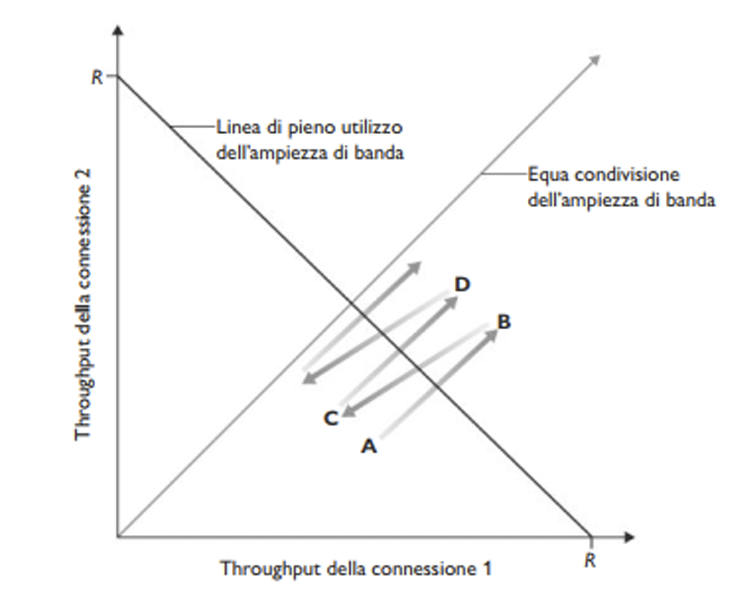
\includegraphics[width=0.65\linewidth]{./images/fairness.png}
\end{figure}

A parità di $RTT$ e $MSS$, gli host \textbf{in congestion avoidance crescono in maniera lineare}: 1 $MSS$ ad ogni $RTT$. Detto ciò, quando la somma del throughput di entrambi gli host supera $R$, questi \textbf{si dimezzano}. Con $x = \text{throughput del primo host}$ e $y = \text{throughput del secondo host}$, e il comportamento di incremento lineare e divisione della finestra di congestione, \textbf{il throughput delle connessioni convergerà sempre alla bisettrice} $x=y$.
In circostanze più vicine a quelle reali, le connessioni con $RTT$ più basso ottengono un throughput maggiore a causa della velocità con cui possono ottenere la connessione. Ricordiamo che l'incremento, nella fase di congestion avoidance, avviene una volta per $RTT$. 
